\ylDisplay{Heelium} % Ülesande nimi
{Tundmatu autor} % Autor
{lahtine} % Voor
{2008} % Aasta
{G 6} % Ülesande nr.
{5} % Raskustase
{
% Teema: Gaasid
\ifStatement
Kolme mooli heeliumi soojendamisel muutus gaasi rõhk võrdeliselt gaasi ruumalaga. Mitme kraadi võrra tõusis heeliumi temperatuur, kui gaasile anti soojushulk $Q = \SI{300}{J}$?
\fi


\ifHint
Paisumisel gaasi poolt tehtud tööd on kõige lihtsam leida $p-V$ graafikult protsessi aluse ala pindalana. Lisaks tuleb kasuks termodünaamika I seadus.
\fi


\ifSolution
\begin{wrapfigure}{r}{0.4\textwidth}
	\begin{center}
		\vspace{-25pt}
		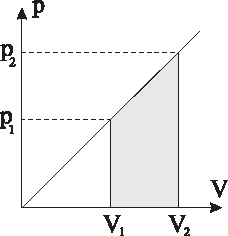
\includegraphics[width=0.95\linewidth]{2008-lahg-06-lah}
	\end{center}
\end{wrapfigure}
Käsitleme heeliumit üheaatomilise ideaalse gaasina. 
Paneme kirja olekuvõrrandid alg- ja lõppseisundi jaoks:
\[
p_1V_1 = nRT_1, \quad p_2V_2 = nRT_2.
\]
Paisumisel tehtav töö võrdub graafikul halliks värvitud
trapetsi pindalaga:
\[
A = \frac 12 (p_2V_2 - p_1V_1) = \frac 12 nR(T_2 - T_1).
\]
Termodünaamika I seaduse kohaselt 
\[
Q = A + \Delta U = \frac 12 nR(T_2 - T_1) + \frac 32 nR\Delta T = 2nR\Delta T.
\]
Siit
\[
\Delta T =\frac {Q}{2nR} \approx \SI{6}{K}.
\]
\fi
}